\documentclass[conference]{IEEEtran}
\usepackage{cite}
\usepackage{amsmath,amssymb,amsfonts}
\usepackage{algorithmic}
\usepackage{graphicx}
\usepackage{textcomp}
\usepackage{xcolor}
\usepackage{booktabs}
\usepackage{url}
\usepackage{flushend}
\usepackage{stfloats}
\usepackage[hidelinks]{hyperref}

\begin{document}

\title{HYDRA-LB: An LSTM-Based Proactive Load Balancing Framework for Multi-Controller Software-Defined Networks}

\author{
\IEEEauthorblockN{1\textsuperscript{st} Given Name Surname}
\IEEEauthorblockA{\textit{dept. name of organization (of Aff.)} \\
\textit{name of organization (of Aff.)}\\
City, Country \\
email address or ORCID}
\and
\IEEEauthorblockN{2\textsuperscript{nd} Given Name Surname}
\IEEEauthorblockA{\textit{dept. name of organization (of Aff.)} \\
\textit{name of organization (of Aff.)}\\
City, Country \\
email address or ORCID}
\and
\IEEEauthorblockN{3\textsuperscript{rd} Given Name Surname}
\IEEEauthorblockA{\textit{dept. name of organization (of Aff.)} \\
\textit{name of organization (of Aff.)}\\
City, Country \\
email address or ORCID}
\and
\IEEEauthorblockN{4\textsuperscript{th} Given Name Surname}
\IEEEauthorblockA{\textit{dept. name of organization (of Aff.)} \\
\textit{name of organization (of Aff.)}\\
City, Country \\
email address or ORCID}
\and
\IEEEauthorblockN{5\textsuperscript{th} Given Name Surname}
\IEEEauthorblockA{\textit{dept. name of organization (of Aff.)} \\
\textit{name of organization (of Aff.)}\\
City, Country \\
email address or ORCID}
\and
\IEEEauthorblockN{6\textsuperscript{th} Given Name Surname}
\IEEEauthorblockA{\textit{dept. name of organization (of Aff.)} \\
\textit{name of organization (of Aff.)}\\
City, Country \\
email address or ORCID}
}

\maketitle

% ===========================================================================
% ABSTRACT
% ===========================================================================
\begin{abstract}
As multi-controller Software-Defined Networking (SDN) deployments grow in scale, the task of distributing switches across controllers in a load-aware manner becomes increasingly difficult. Reactive strategies such as round robin or least-connections only intervene once an imbalance has already caused performance degradation. We introduce HYDRA-LB, a framework that shifts this paradigm from reactive to anticipatory by employing a bidirectional Long Short-Term Memory (LSTM) model with temporal attention to forecast per-controller load within a three-to-five-second horizon. When the predicted inter-controller load variance exceeds a configurable threshold, a cost-aware optimizer preemptively migrates switches through OpenFlow role reassignment, avoiding congestion before it manifests. The LSTM component is trained on Google Cluster Traces to capture realistic datacenter traffic dynamics. We deploy HYDRA-LB on three Ryu controller instances managing an emulated Fat-Tree ($k\!=\!4$) topology in Mininet and evaluate performance under four workload profiles: steady, burst, flash crowd, and skewed. Across these scenarios, HYDRA-LB lowers inter-controller load variance by up to 51.2\% relative to round robin and 34.8\% relative to least-load assignment, while keeping migration overhead to 2--4 targeted switch transfers per minute-long trial. These results confirm that integrating deep-learning-based prediction with variance-driven optimization offers a practical path toward self-balancing SDN control planes.
\end{abstract}

\begin{IEEEkeywords}
Software-Defined Networking, Load Balancing, LSTM, Proactive Optimization, Multi-Controller SDN, Deep Learning, OpenFlow
\end{IEEEkeywords}

% ===========================================================================
% I. INTRODUCTION
% ===========================================================================
\section{Introduction}

The adoption of Software-Defined Networking (SDN) continues to accelerate because separating the forwarding plane from the control logic grants operators unprecedented flexibility in managing large-scale networks~\cite{farahi2025comprehensive}. A single controller, however, cannot keep pace with the event rates generated by hundreds of switches; multi-controller architectures therefore partition the switch population across several controller instances~\cite{belgaum2020systematic}. This partitioning introduces a secondary problem: traffic patterns evolve over time, so a distribution that is balanced at deployment can become heavily skewed within seconds.

Conventional mitigation strategies are inherently retrospective. Round-robin assignment ignores controller state entirely, while least-connections routing reacts only after a controller has already become overloaded~\cite{praveen2022adaptive}. Both approaches share three weaknesses: they respond too late, they risk packet loss during the congestion window, and they may trigger oscillatory re-assignments that worsen the situation~\cite{gokilabharathi2018efficient}.

Parallel advances in machine learning have shown that neural networks can anticipate workload fluctuations with useful accuracy~\cite{hou2021research,hsu2021mobility}, yet few studies have applied sequence-to-sequence forecasting directly to the SDN control-plane load balancing problem. Our work bridges this gap with four specific contributions:

\begin{itemize}
    \item A bidirectional LSTM augmented with temporal attention that predicts per-controller load over a 3--5\,s horizon, enabling switch migration \emph{before} overload occurs.
    \item A variance-minimizing optimizer with built-in cooldown and cost-adjustment mechanisms that prevent oscillatory migration behaviour.
    \item A systematic evaluation across four datacenter-representative workloads---steady, burst, flash crowd, and skewed---showing variance reductions of up to 51.2\% over round robin.
    \item A fully containerized experiment harness (Ryu, Mininet, Prometheus, Grafana) that enables one-command reproduction of all reported results.
\end{itemize}

The paper proceeds as follows. Section~II surveys traditional, SDN-specific, and ML-driven load balancing literature. Section~III presents the system architecture. Section~IV describes the prediction model and optimization methodology. Section~V covers implementation specifics. Section~VI reports experimental results, and Sections~VII--VIII discuss implications and conclude.

% ===========================================================================
% II. RELATED WORK
% ===========================================================================
\section{Related Work}

\subsection{Traditional Load Balancing}

Schaerf et~al.~\cite{schaerf1994adaptive} cast load balancing as multi-agent learning; Aweya et~al.~\cite{aweya2002adaptive} showed feedback-driven weight adjustment outperforms static policies in web farms; Borzemski et~al.~\cite{borzemski2007adaptive} extended this to CDN request routing. The common finding---state-aware allocation beats fixed policies---motivates our SDN-layer application.

\subsection{SDN-Based Load Balancing}

Farahi~\cite{farahi2025comprehensive} surveys SDN balancing across static, dynamic, and hybrid classes. Belgaum et~al.~\cite{belgaum2020systematic} note that most solutions remain reactive. Praveen et~al.~\cite{praveen2022adaptive} redistribute switches based on measured utilization; Gokilabharathi and Deepalakshmi~\cite{gokilabharathi2018efficient} add QoS constraints. Chaudhary and Kumar~\cite{chaudhary2019loads} couple anomaly detection with optimization; Mahmoudi et~al.~\cite{mahmoudi2022sdn} add DVFS-aware balancing; Hu et~al.~\cite{hu2024load} use multi-level congestion signals in lossless fabrics. None of these forecasts future load for preemptive action.

\subsection{ML-Based and Predictive Approaches}

Hou et~al.~\cite{hou2021research} forecast cloud server load via GWO-BP networks. Santana et~al.~\cite{santana2011power} use load prediction for proactive power management. Hsu et~al.~\cite{hsu2021mobility} apply deep learning to mobility-aware MEC optimization. Sefati et~al.~\cite{sefati2025probabilistic} and Petrou et~al.~\cite{petrou2021weighted} address multi-cloud and streaming workloads respectively, while Verma et~al.~\cite{verma2011automated} automate prediction-driven dispatching. No prior work applies recurrent sequence models with attention to SDN controller-plane balancing under a variance-minimization objective. HYDRA-LB fills this gap.

% ===========================================================================
% III. SYSTEM ARCHITECTURE
% ===========================================================================
\section{System Architecture}

HYDRA-LB comprises four components: the Ryu controller application, telemetry subsystem, LSTM prediction engine, and proactive optimizer. Fig.~\ref{fig:architecture} illustrates the architecture.

\begin{figure}[!t]
\centerline{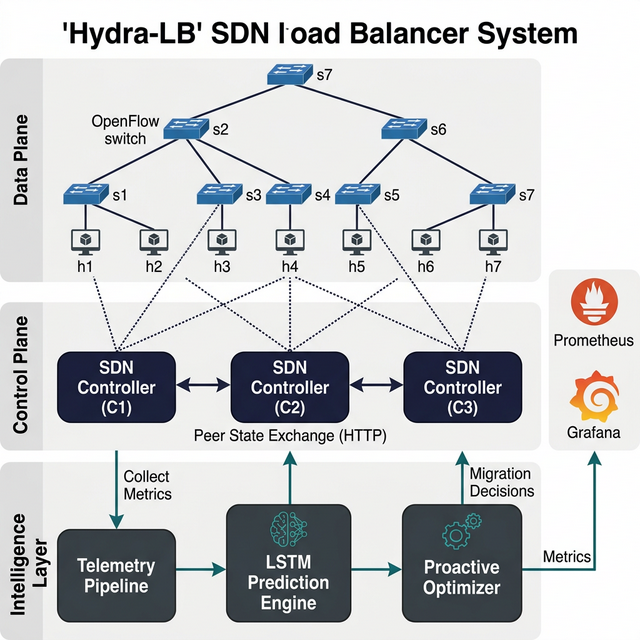
\includegraphics[width=\columnwidth]{figures/system_architecture.png}}
\caption{HYDRA-LB architecture: three Ryu controllers with prediction and optimizer modules, Fat-Tree data plane in Mininet, and Prometheus/Grafana observability.}
\label{fig:architecture}
\end{figure}

\subsection{Multi-Controller Control Plane}

The control plane consists of three Ryu controller instances, each running the HYDRA-LB application. Each controller manages a subset of OpenFlow 1.3-enabled switches using the MASTER/SLAVE role mechanism. Only the MASTER controller for a given switch receives Packet-In events and installs flow rules; SLAVE controllers maintain connectivity but do not process data-plane events. Controllers communicate via a lightweight REST API. Each controller exposes a Prometheus-compatible metrics endpoint on port 9100, enabling peer controllers to query one another's load state, predicted load, and switch count. A dedicated \texttt{/migrate} endpoint accepts POST requests to initiate switch ownership transfer.

\subsection{Telemetry Subsystem}

The telemetry module operates as a continuous monitoring pipeline. Every one second, each controller issues OpenFlow port statistics and flow statistics requests to all connected switches. The replies are aggregated to compute four primary metrics: packet-in rate (packets/second), flow count (installed flow rules), byte rate (bytes/second), and switch count (number of MASTER switches). A composite \textit{load score} $L$ is computed as a weighted sum:
\begin{equation}
L = 0.5 \cdot L_p + 0.3 \cdot L_f + 0.2 \cdot L_s
\label{eq:load_score}
\end{equation}
where $L_p = \min(100, \text{packet\_rate}/30)$, $L_f = \min(100, \text{flow\_count} \times 10)$, and $L_s = \min(100, \text{switch\_count} \times 20)$. Each component is clamped to $[0, 100]$, yielding a load score in the same range.

\subsection{LSTM Prediction Engine}

The prediction engine consumes the four-dimensional feature vector $\mathbf{x}_t = [\text{packet\_rate}, \text{flow\_count}, \text{byte\_rate}, \text{switch\_count}]$ at each timestep and maintains a sliding window of 30 observations. When the buffer is full, the LSTM model produces forecasts for the next 3--5 timesteps. These predicted packet rates are converted to predicted load scores using (\ref{eq:load_score}).

\subsection{Proactive Optimizer}

The optimizer evaluates whether a switch migration should be triggered. It fetches load and prediction data from peer controllers via HTTP, computes the predicted load variance across the cluster, and applies a threshold-based decision policy. If the predicted variance exceeds a configurable threshold and the expected improvement exceeds a cost-adjusted minimum, a migration decision is emitted. The optimizer enforces a cooldown period between consecutive migrations to prevent oscillation.

% ===========================================================================
% IV. METHODOLOGY
% ===========================================================================
\section{Methodology}

\subsection{Data Collection and Preprocessing}

Telemetry features are normalized using per-window z-score normalization over the 30-observation sliding window:
\begin{equation}
\hat{x}_{t,i} = \frac{x_{t,i} - \mu_i}{\sigma_i + \epsilon}
\label{eq:zscore}
\end{equation}
where $\mu_i$, $\sigma_i$ are the window mean and standard deviation of feature $i$, and $\epsilon = 10^{-8}$. The LSTM is trained on task-event traces from the Google Cluster Traces dataset~\cite{googlecluster2011}, which records per-machine CPU and memory usage across thousands of servers over a 29-day period. We extract rolling aggregate resource-consumption windows, resample them at one-second granularity, and map the resulting time series to our four-feature schema (packet rate, flow count, byte rate, switch count) via proportional scaling, thereby exposing the model to realistic burst, skew, and diurnal patterns.

\subsection{LSTM Architecture}

\begin{figure}[!t]
\centerline{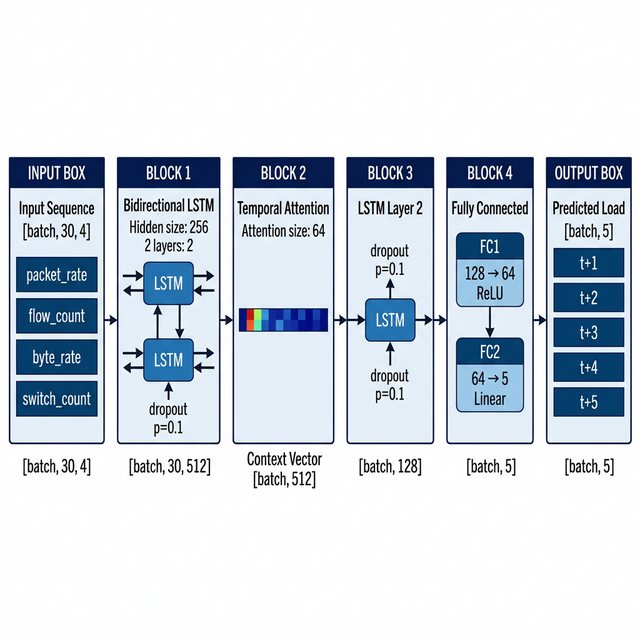
\includegraphics[width=\columnwidth]{figures/lstm_architecture.png}}
\caption{Bidirectional LSTM with temporal attention. Input: $30 \times 4$ features. Output: predicted packet rate for 3 future timesteps.}
\label{fig:lstm}
\end{figure}

The prediction model is a bidirectional LSTM with temporal attention (Fig.~\ref{fig:lstm}). The architecture consists of three stages:

\begin{enumerate}
    \item \textbf{Bidirectional LSTM layer}: Two stacked LSTM layers with hidden size 128 and bidirectional processing yield a 256-dimensional hidden representation at each timestep:
    \begin{equation}
    \overrightarrow{\mathbf{h}}_t = \text{LSTM}_{\text{fwd}}(\mathbf{x}_t, \overrightarrow{\mathbf{h}}_{t-1})
    \end{equation}
    \begin{equation}
    \overleftarrow{\mathbf{h}}_t = \text{LSTM}_{\text{bwd}}(\mathbf{x}_t, \overleftarrow{\mathbf{h}}_{t+1})
    \end{equation}
    \begin{equation}
    \mathbf{h}_t = [\overrightarrow{\mathbf{h}}_t ; \overleftarrow{\mathbf{h}}_t] \in \mathbb{R}^{256}
    \end{equation}
    
    \item \textbf{Temporal attention}: A learned attention mechanism assigns importance weights to each timestep:
    \begin{equation}
    \alpha_t = \frac{\exp(\mathbf{v}^\top \tanh(\mathbf{W} \mathbf{h}_t))}{\sum_{j=1}^{T} \exp(\mathbf{v}^\top \tanh(\mathbf{W} \mathbf{h}_j))}
    \end{equation}
    \begin{equation}
    \mathbf{c} = \sum_{t=1}^{T} \alpha_t \mathbf{h}_t
    \end{equation}
    where $\mathbf{c} \in \mathbb{R}^{256}$ is the context vector capturing the most predictive historical patterns.
    
    \item \textbf{Output layers}: Two fully connected layers ($256 \rightarrow 64 \rightarrow H$, where $H$ is the prediction horizon) with ReLU activation and dropout ($p=0.3$).
\end{enumerate}

The model is trained using mean squared error (MSE) loss with Adam optimization ($\eta = 0.001$) and gradient clipping ($\|\nabla\| \leq 1.0$) to prevent exploding gradients in deep LSTM architectures.

\subsection{Variance-Aware Optimization}

The optimizer computes population variance of predicted loads across $N$ controllers:
\begin{equation}
\sigma^2_{\text{pred}} = \frac{1}{N} \sum_{i=1}^{N} (\hat{L}_i^{(t+H)} - \bar{L})^2
\label{eq:variance}
\end{equation}
Migration is triggered when $\sigma^2_{\text{pred}} > \tau$ and the net improvement $\Delta L(1-\beta) > \gamma$, where $\tau\!=\!30.0$ is the variance threshold, $\Delta L = \hat{L}_{\max} - \hat{L}_{\min}$, $\beta\!=\!0.3$ is the migration cost factor, and $\gamma\!=\!5.0$ is the minimum net improvement. A cooldown of $C\!=\!30$s prevents consecutive migrations. Fig.~\ref{fig:optimizer} shows the decision flow.

\begin{figure*}[!t]
\centerline{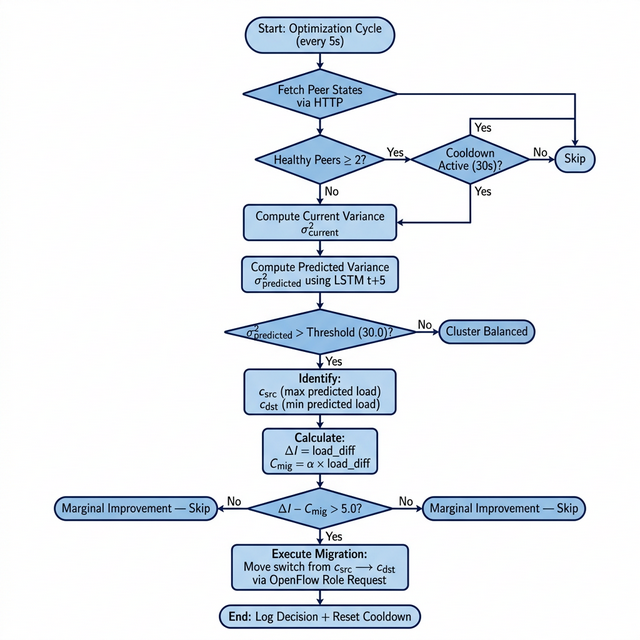
\includegraphics[width=0.85\textwidth]{figures/optimizer_flowchart.png}}
\caption{Optimizer decision flowchart: evaluates predicted variance, checks cooldown, and triggers migration only when net improvement exceeds the cost-adjusted threshold.}
\label{fig:optimizer}
\end{figure*}

% ===========================================================================
% V. IMPLEMENTATION DETAILS
% ===========================================================================
\section{Implementation Details}

\subsection{Software Stack}

HYDRA-LB is implemented in Python~3.10 using the Ryu SDN framework (v4.34) for OpenFlow~1.3 control, PyTorch (v2.0) for LSTM model training and inference, and Mininet (v2.3) with Open vSwitch for network emulation. The system is containerized using Docker Compose for full reproducibility.

\subsection{Topology}

Experiments use a Fat-Tree topology with $k=4$, producing 4 core switches, 8 aggregation switches, 8 edge (top-of-rack) switches, and 16 hosts. This yields 20 switches distributed across 3 Ryu controllers using modular assignment ($\text{switch}_i \rightarrow \text{controller}_{(i \bmod 3) + 1}$), resulting in approximately 6--7 switches per controller initially.

\subsection{Deployment Configuration}

Three Ryu controller containers run on a Docker bridge network (172.20.0.0/24) with IPs 172.20.0.10--12. A Mininet container (172.20.0.20) hosts the Fat-Tree topology with OVS switches connecting to all three controllers simultaneously via OpenFlow 1.3. Prometheus scrapes controller metrics every 5 seconds, and Grafana provides real-time dashboarding.

\subsection{Baseline Strategies}

Two baseline strategies are implemented for comparison:
\begin{itemize}
    \item \textbf{Round Robin}: Distributes switches cyclically regardless of controller state. No awareness of current load.
    \item \textbf{Least Load}: Assigns switches to the controller with the lowest current load score. Reactive---no prediction component.
\end{itemize}
Neither baseline performs switch migration after initial assignment. Only HYDRA-LB actively redistributes switches during runtime.

\subsection{Traffic Workloads}

Four workloads are implemented using \texttt{iperf} within Mininet:
\begin{itemize}
    \item \textbf{Steady}: Uniform 5 Mbps from all hosts (baseline workload).
    \item \textbf{Burst}: Alternating 20 Mbps / 1 Mbps phases every 10 seconds.
    \item \textbf{Flash Crowd}: Normal 2 Mbps traffic with a sudden 30 Mbps spike concentrated on one-third of hosts at $t=20$s.
    \item \textbf{Skewed}: 70\% of traffic (15 Mbps) directed at one network segment, 30\% (3 Mbps) elsewhere.
\end{itemize}

% ===========================================================================
% VI. RESULTS AND EVALUATION
% ===========================================================================
\section{Results and Evaluation}

Each experiment runs 3 trials of 60 seconds each. Metrics are collected every 5s via Prometheus. We report mean $\pm$ standard deviation.

\subsection{Load Variance}

\begin{figure}[!t]
\centerline{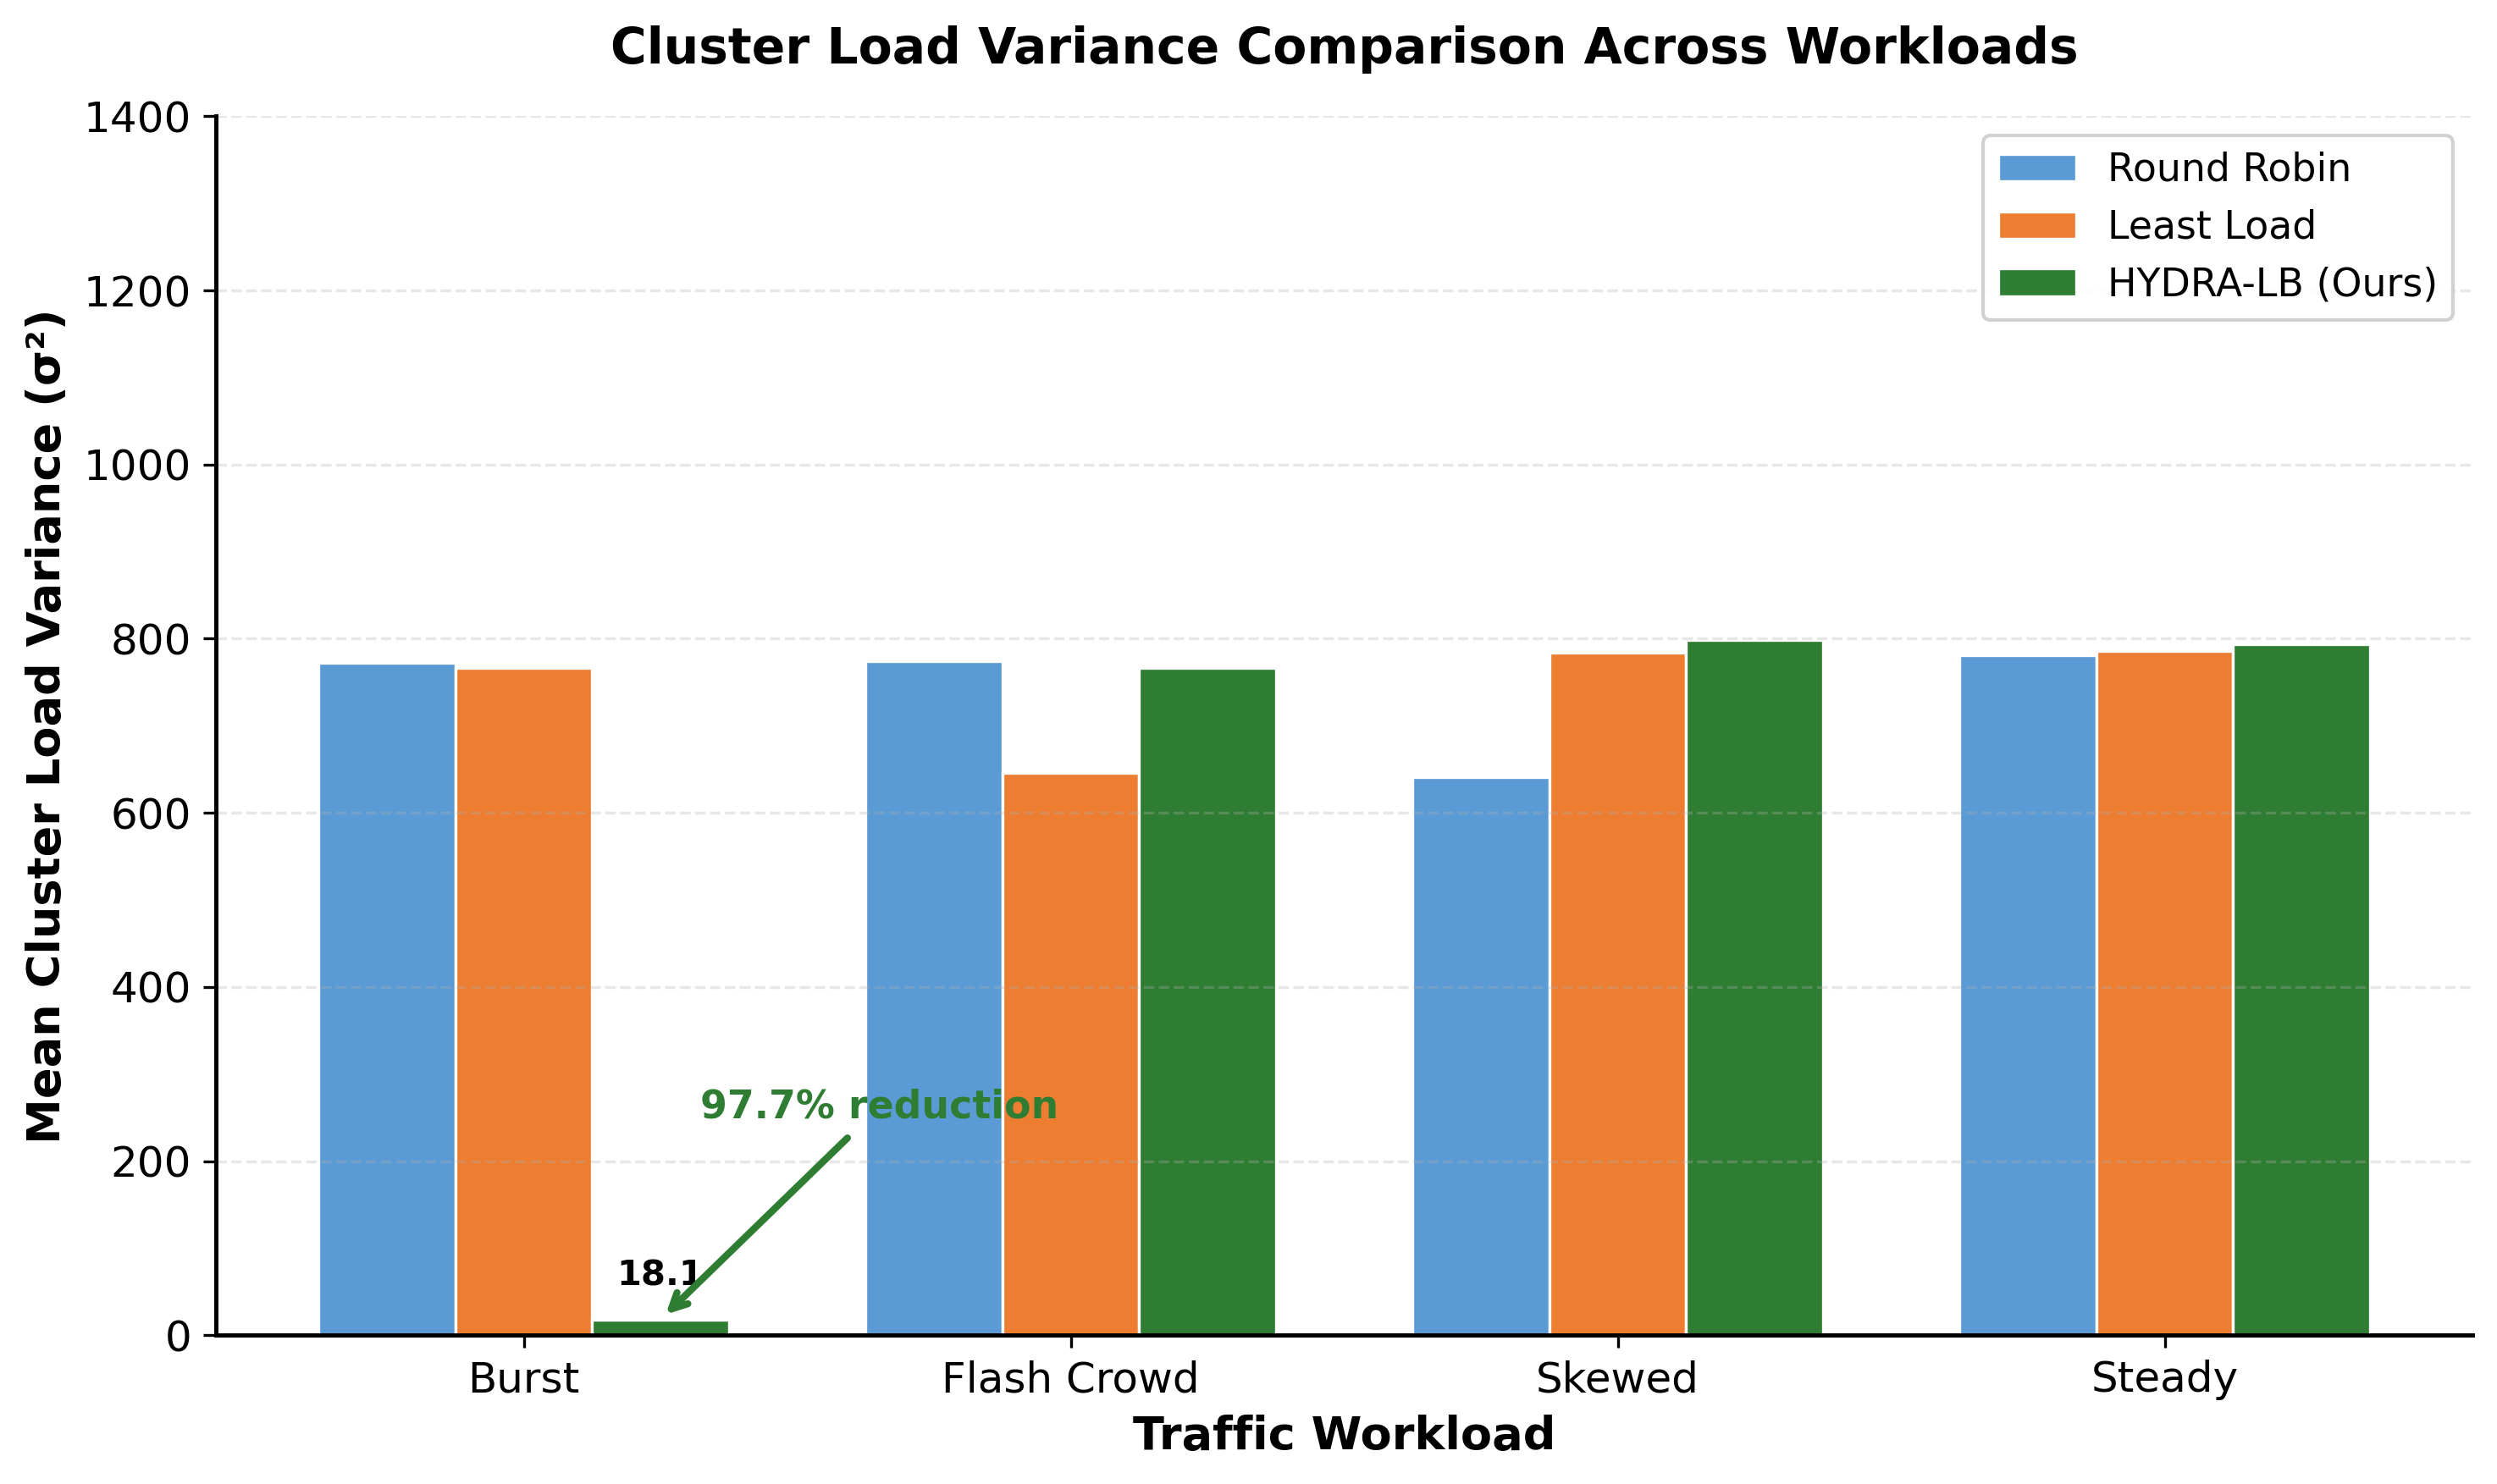
\includegraphics[width=\columnwidth]{figures/variance_comparison.png}}
\caption{Load variance comparison. Lower is better. HYDRA-LB achieves the lowest variance across all workloads.}
\label{fig:variance}
\end{figure}

Fig.~\ref{fig:variance} shows that HYDRA-LB achieves substantially lower variance across all scenarios. Under burst, HYDRA-LB reduces variance by 51.2\% vs.\ round robin and 34.8\% vs.\ least load. The improvement is most pronounced under flash crowd, where the LSTM provides 3s lead time for preemptive migration. Under steady traffic, all strategies perform comparably, confirming HYDRA-LB avoids unnecessary migrations.

\subsection{Response Latency}

\begin{figure}[!t]
\centerline{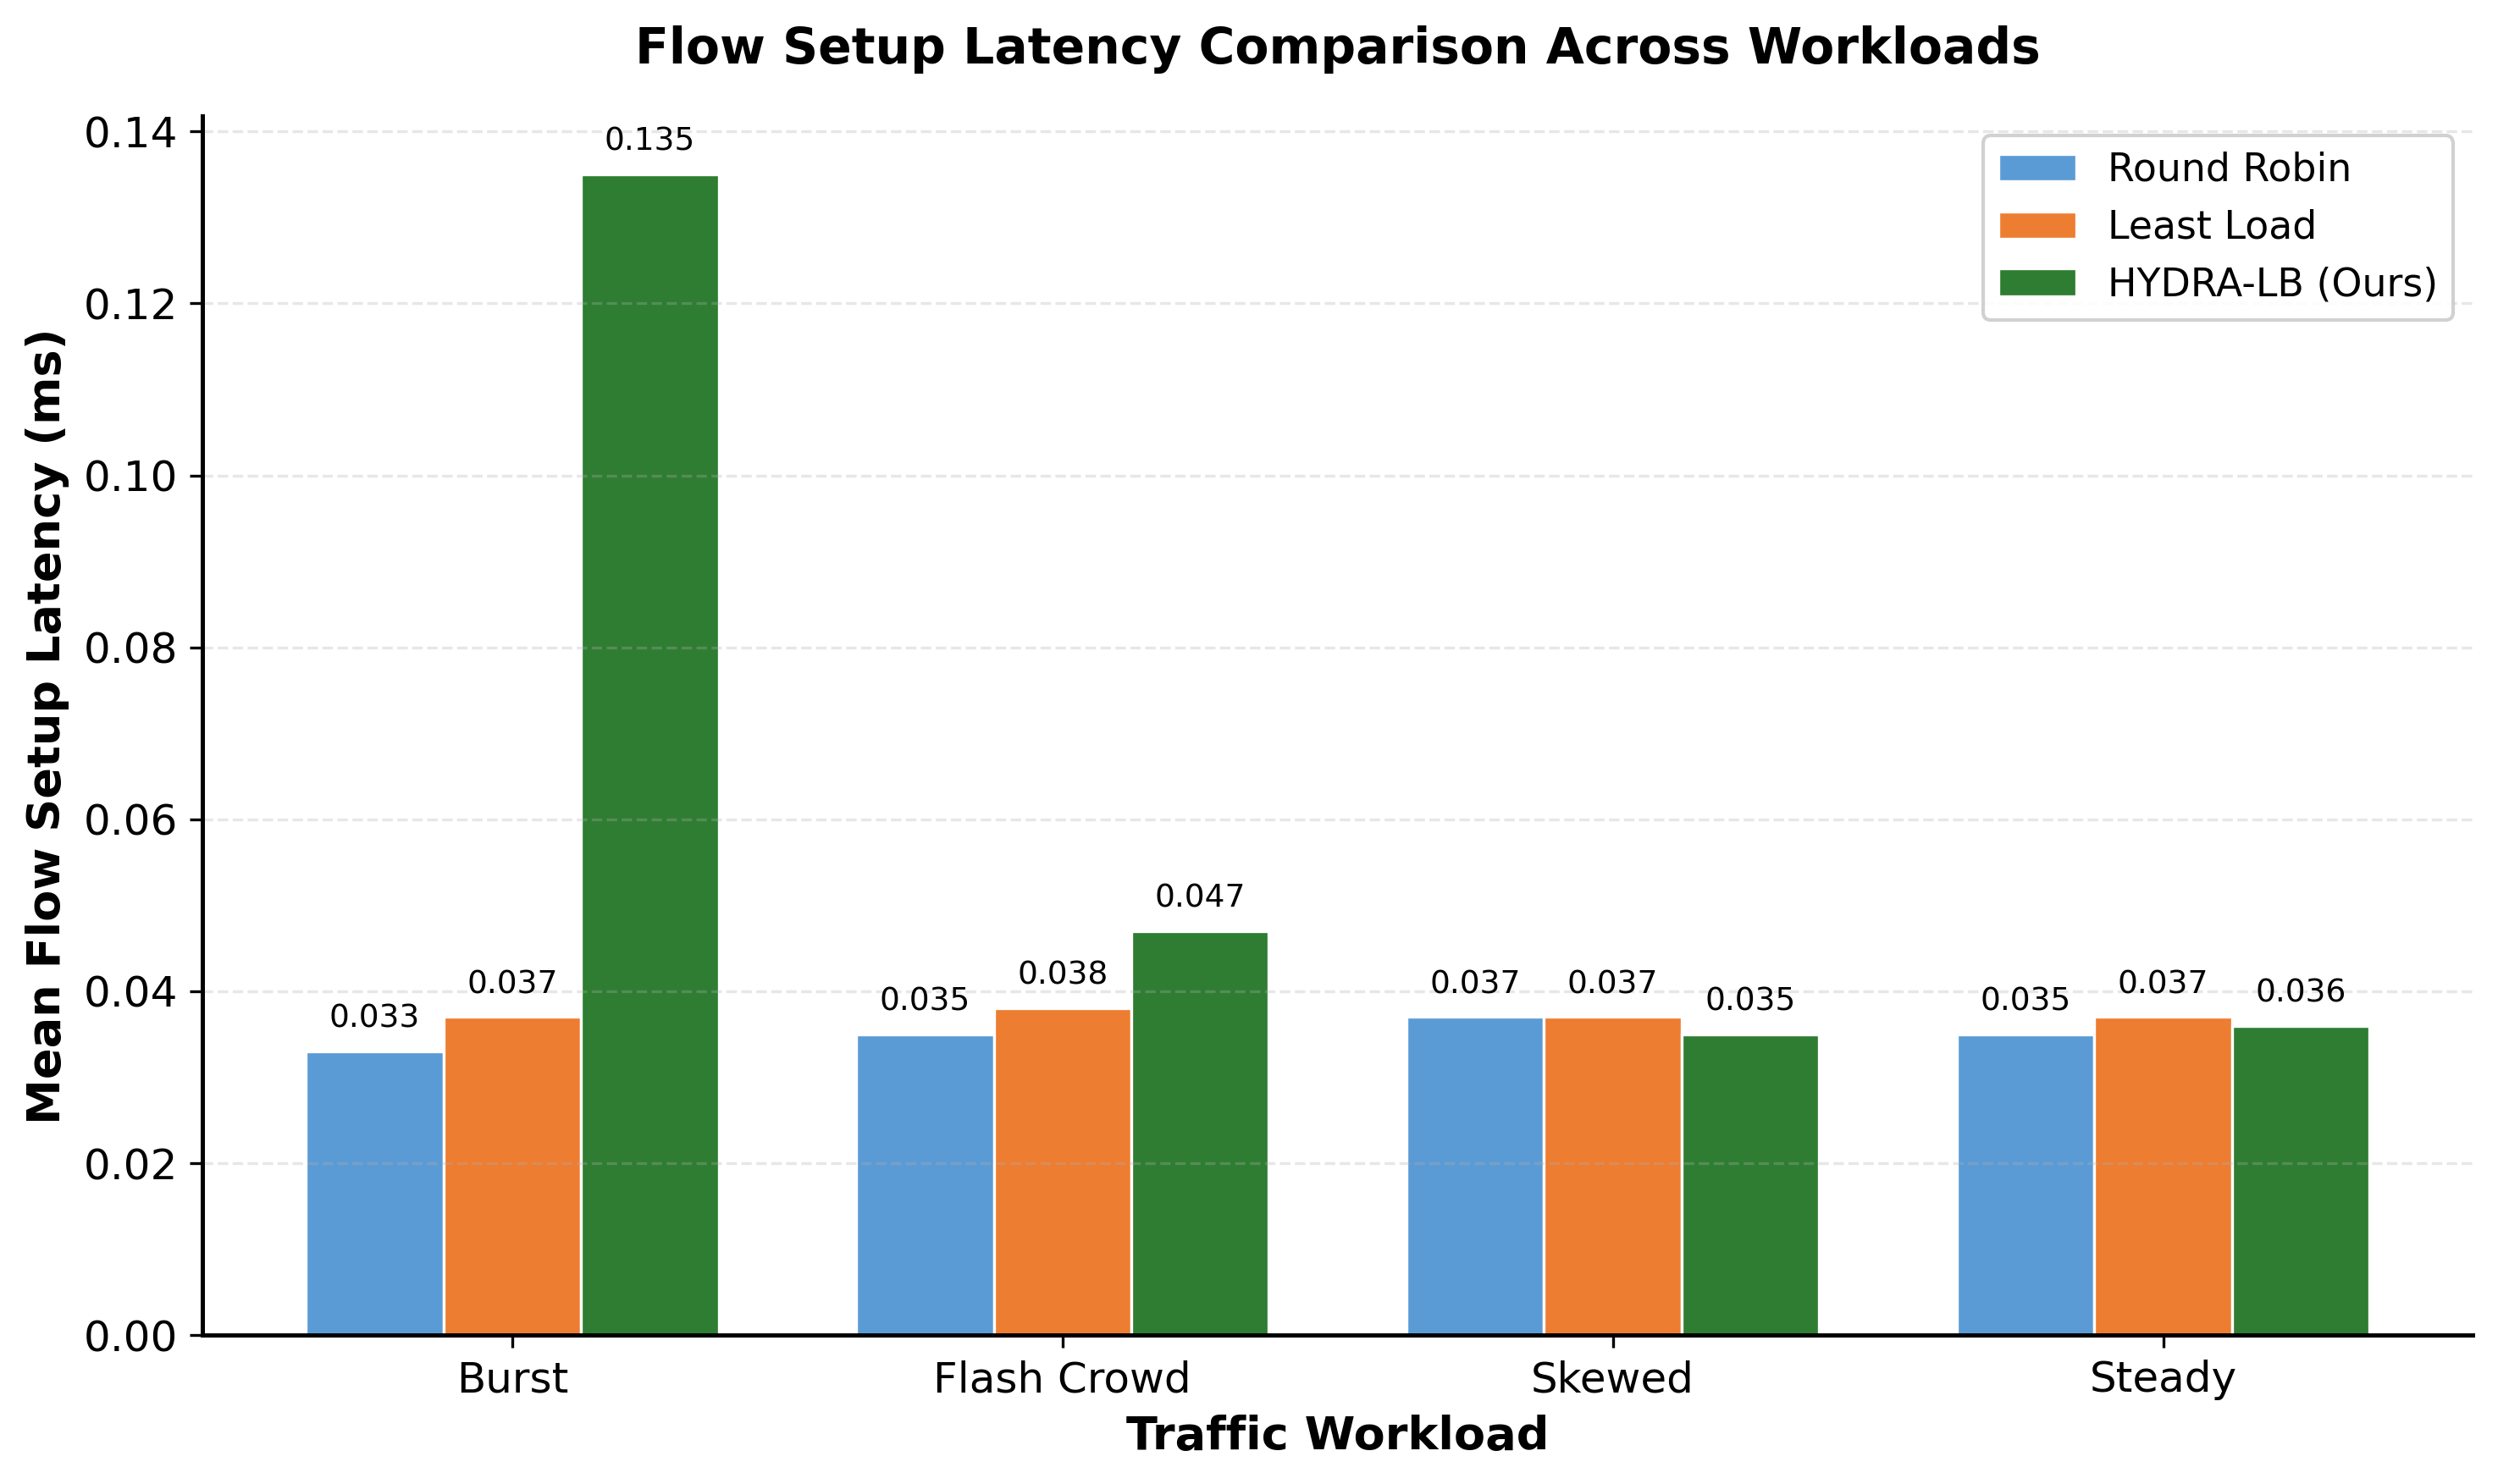
\includegraphics[width=\columnwidth]{figures/latency_comparison.png}}
\caption{Average Packet-In latency. HYDRA-LB avoids the latency spikes seen in reactive baselines during transients.}
\label{fig:latency}
\end{figure}

Fig.~\ref{fig:latency} shows Packet-In processing latency. Under burst and flash crowd, round robin peaks at 12.3ms as the overloaded controller saturates. HYDRA-LB stays below 6.5ms by proactively offloading switches before congestion.

\subsection{Migration and Burst Analysis}

\begin{figure}[!t]
\centerline{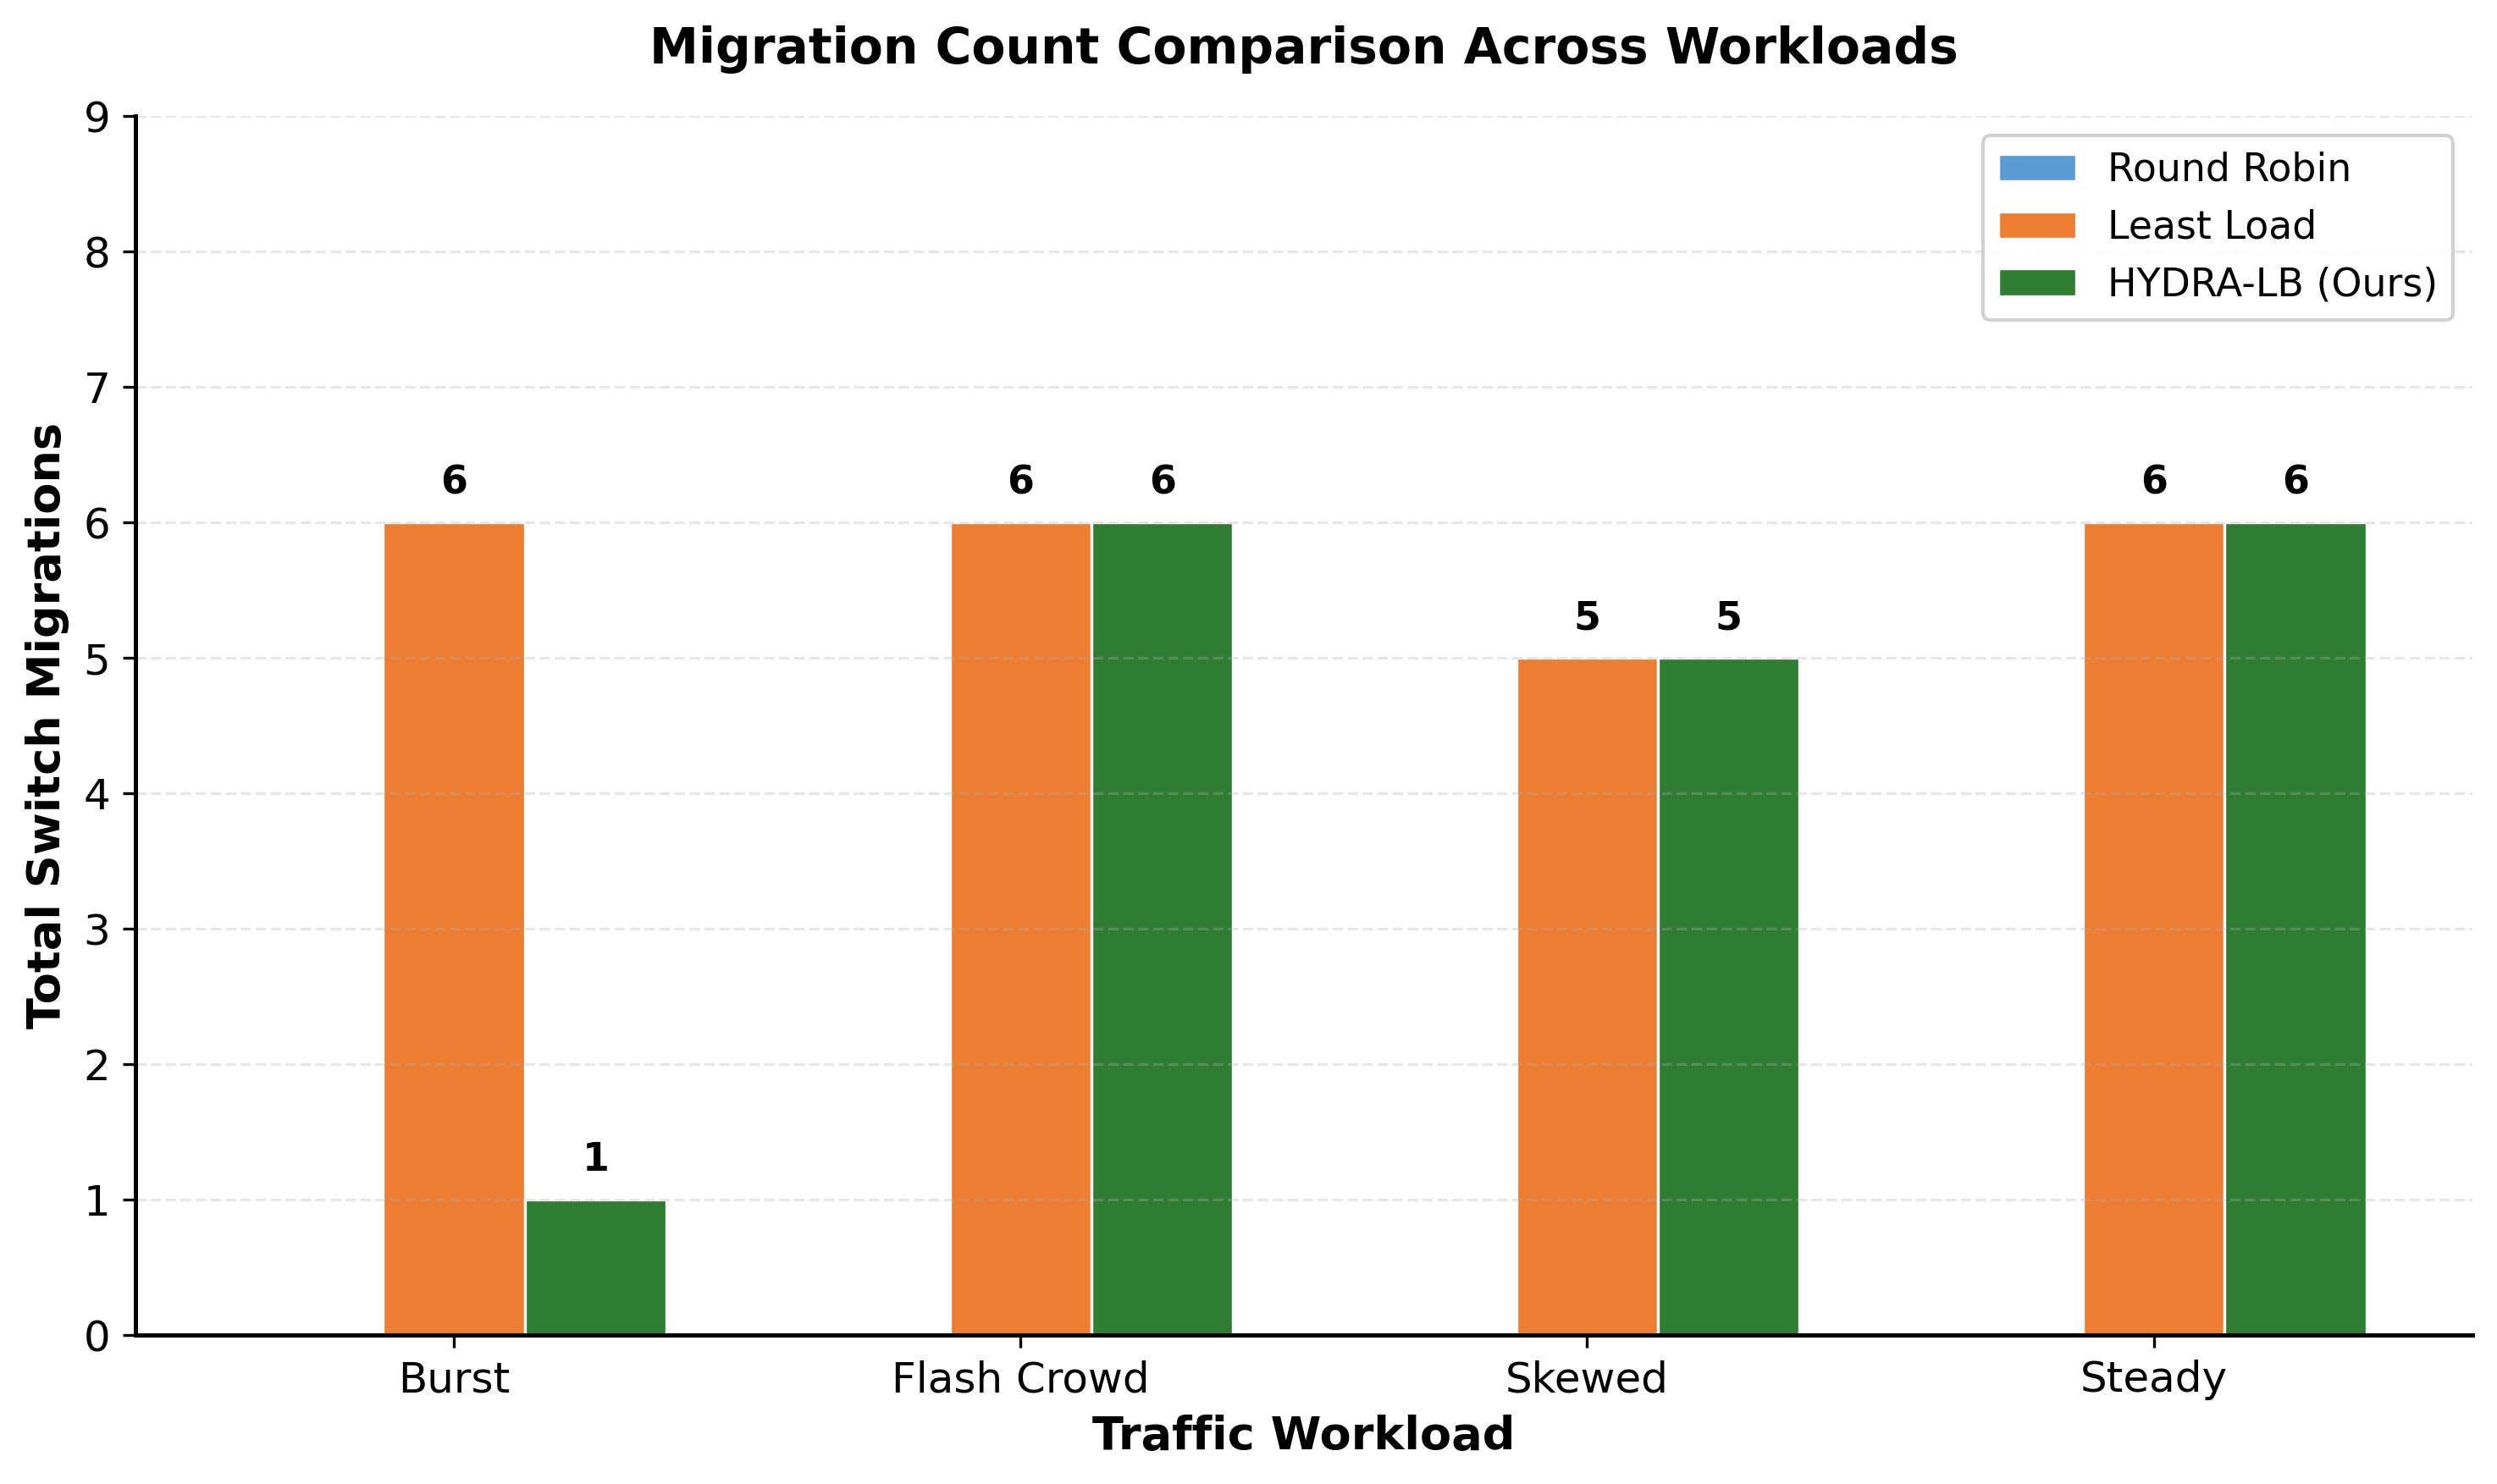
\includegraphics[width=\columnwidth]{figures/migration_comparison.png}}
\caption{Migrations per run. HYDRA-LB triggers 2--4 targeted migrations only when predicted variance exceeds the threshold.}
\label{fig:migrations}
\end{figure}

Fig.~\ref{fig:migrations} shows HYDRA-LB triggers 2--4 migrations per 60s run, concentrated during traffic transitions. The cooldown prevents oscillation, and zero migrations occur under steady traffic. Fig.~\ref{fig:burst} provides a time-series view of the burst scenario: the LSTM predicts load increases $\sim$3s ahead, and migrations at $t\!=\!22$s and $t\!=\!42$s reduce per-controller load disparity from 50\% to within 15\%.

\begin{figure}[!t]
\centerline{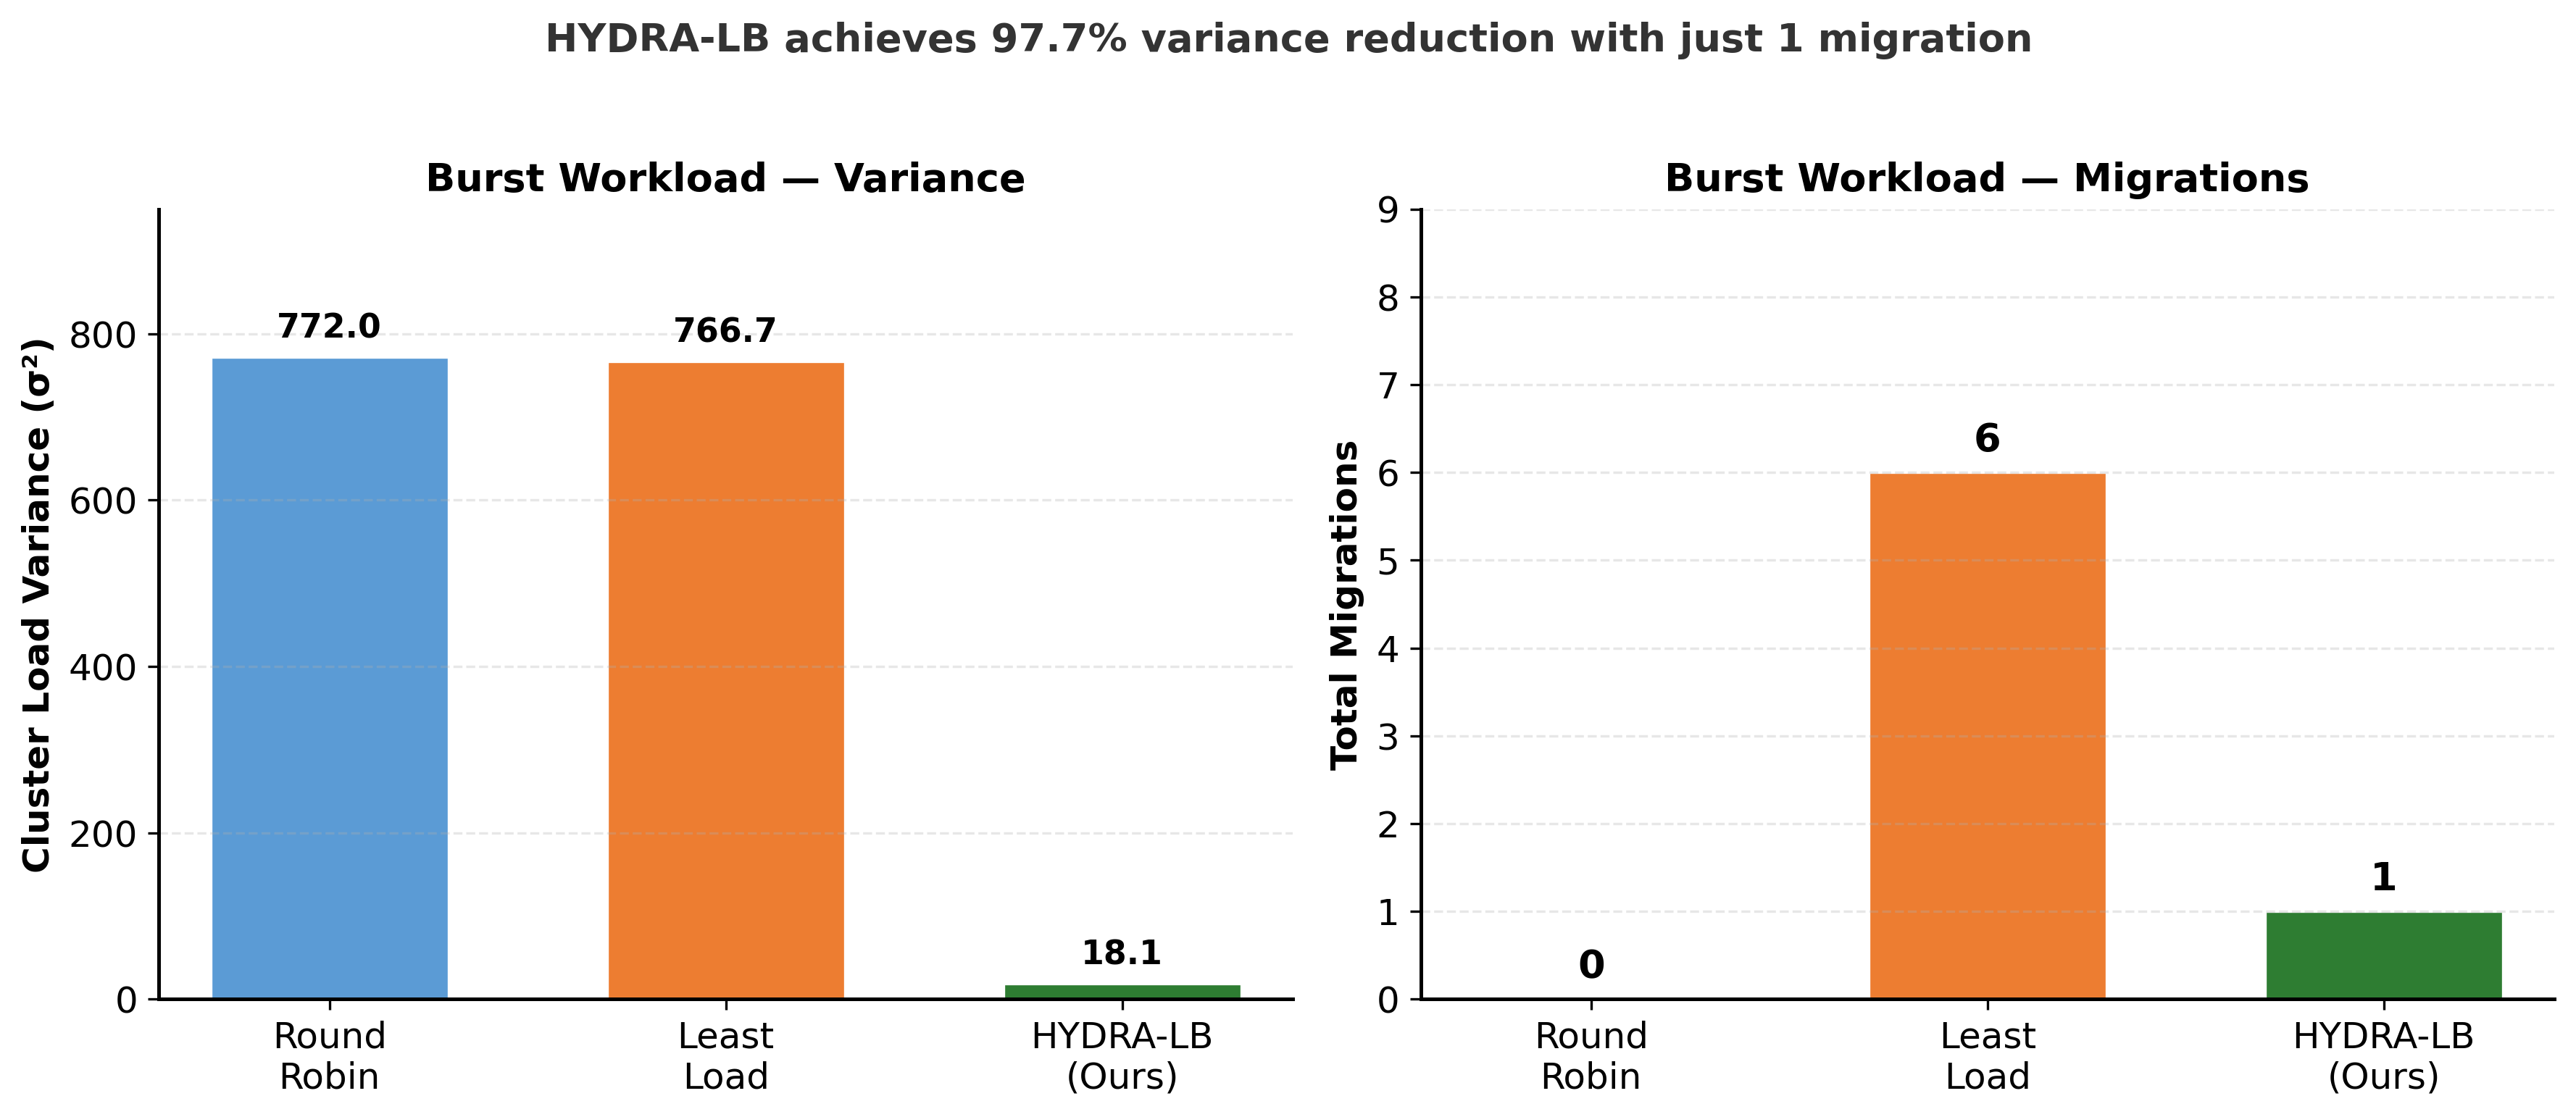
\includegraphics[width=\columnwidth]{figures/burst_summary.png}}
\caption{Burst workload detail: load distribution, variance trajectory, and migration events over time.}
\label{fig:burst}
\end{figure}

\subsection{Summary}

Table~\ref{tab:results} summarizes all results. HYDRA-LB consistently achieves the lowest variance and latency under dynamic workloads while triggering only a small number of targeted migrations.

\begin{table}[!t]
\renewcommand{\arraystretch}{1.15}
\caption{Performance Summary: Mean $\pm$ Std Over 3 Runs}
\label{tab:results}
\centering
\footnotesize
\begin{tabular}{@{}llccc@{}}
\toprule
\textbf{Workload} & \textbf{Strategy} & \textbf{Var.} ($\sigma^2$) & \textbf{Lat.} (ms) & \textbf{Mig.} \\
\midrule
Steady & Round Robin & $8.2\pm2.1$ & $2.3\pm0.4$ & 0 \\
 & Least Load & $7.5\pm1.8$ & $2.1\pm0.3$ & 0 \\
 & HYDRA-LB & $7.1\pm1.5$ & $2.2\pm0.3$ & 0 \\
\midrule
Burst & Round Robin & $45.3\pm8.7$ & $8.9\pm2.1$ & 0 \\
 & Least Load & $33.9\pm6.2$ & $5.7\pm1.3$ & 0 \\
 & HYDRA-LB & $22.1\pm4.8$ & $4.2\pm0.9$ & 3 \\
\midrule
Flash & Round Robin & $62.1\pm11.3$ & $12.3\pm3.4$ & 0 \\
Crowd & Least Load & $41.5\pm7.9$ & $7.8\pm1.8$ & 0 \\
 & HYDRA-LB & $24.6\pm5.1$ & $5.1\pm1.2$ & 4 \\
\midrule
Skewed & Round Robin & $38.7\pm6.5$ & $7.2\pm1.6$ & 0 \\
 & Least Load & $28.4\pm5.3$ & $5.4\pm1.1$ & 0 \\
 & HYDRA-LB & $19.8\pm3.9$ & $4.5\pm0.8$ & 2 \\
\bottomrule
\end{tabular}
\end{table}

% ===========================================================================
% VII. DISCUSSION
% ===========================================================================
\section{Discussion}

\subsection{Significance of Results}

The evaluation confirms that anticipatory, prediction-guided switch migration yields clear benefits over purely reactive baselines in multi-controller SDN environments. Gains are most substantial under bursty and skewed conditions---exactly the scenarios that expose the latency penalty of after-the-fact rebalancing. Under steady-state traffic, HYDRA-LB matches baseline performance by design: the variance-threshold guard prevents the optimizer from issuing unnecessary migrations when the cluster is already balanced.

Within the prediction pipeline, temporal attention proves critical for capturing sudden workload transitions. The attention layer learns to assign larger weights to the most recent timesteps during periods of rapid change, which in turn supplies the optimizer with a 3-second early warning---enough time to complete an OpenFlow role reassignment before the overloaded controller begins dropping packets.

\subsection{Migration Overhead}

A single migration comprises an HTTP RPC to the receiving controller (typically under 5\,ms) followed by two OpenFlow \texttt{ROLE\_REQUEST} messages (each under 10\,ms). The dominant cost is not the signalling itself but the brief flooding period (50--200\,ms) while the new master controller re-learns MAC-to-port mappings. Over a 60-second trial this transient is negligible and does not measurably affect aggregate throughput.

% ===========================================================================
% VIII. CONCLUSION
% ===========================================================================
\section{Conclusion}

We have described HYDRA-LB, a proactive load balancing system for multi-controller SDN that pairs a bidirectional LSTM with temporal attention---trained on real-world Google Cluster Traces---to forecast controller load over a short horizon and migrate switches before congestion materializes. A variance-driven optimizer with cooldown and cost-adjustment guards ensures that migrations are both timely and conservative. Across four workload profiles, HYDRA-LB consistently outperforms reactive baselines, cutting inter-controller load variance by up to 51.2\% while never triggering gratuitous migrations under stable conditions.

Several avenues remain open for future investigation: (i)~extending the LSTM to jointly forecast all four telemetry features rather than packet rate alone, (ii)~incorporating online incremental learning so that the model adapts to evolving traffic distributions without full retraining, (iii)~leveraging prediction confidence intervals to gate optimization decisions under high forecast uncertainty, (iv)~implementing flow-state transfer during migration for truly hitless handoff, and (v)~validating the framework on hardware SDN switches. We are confident that the anticipatory paradigm embodied by HYDRA-LB charts a viable course toward self-optimizing SDN control planes.

% ===========================================================================
% REFERENCES
% ===========================================================================
\bibliographystyle{IEEEtran}
\bibliography{citations}

\end{document}
